\documentclass[12pt]{article}
\usepackage[letterpaper,margin=0.7in,headheight=15pt,headsep=16pt,footskip=25pt]{geometry}
\usepackage{tikz,array,fancyhdr,lmodern}
\renewcommand{\familydefault}{\sfdefault}
\pagestyle{fancy}\fancyhf{}\renewcommand{\headrulewidth}{0.35pt}
\fancyhead[L]{\small Week 27 / Stable pairings encore / Grades 2--5}
\fancyfoot[L]{\scriptsize Bellingham Math Circle / Week 27 / W27-BON-v1}\fancyfoot[R]{\scriptsize\thepage}
\setlength{\parindent}{0pt}\setlength{\parskip}{9pt}
\newcommand{\problem}[2]{\par\textbf{Problem #1:} #2\par}
\newcommand{\lines}[1]{\foreach \y in {1,...,#1}{\par\vspace{20pt}\hrule height 0.3pt\relax}}
\newcommand{\strips}[6]{\begin{tabular}{r|l@{\hspace{1.1in}}r|l}A&#1&X&#4\\[8pt]B&#2&Y&#5\\[8pt]C&#3&Z&#6\end{tabular}}
\newcommand{\roommateboard}{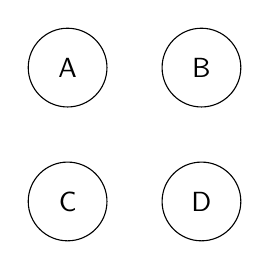
\begin{tikzpicture}[x=1cm,y=1cm]\foreach \l/\x/\y in {A/0/1.7,B/1.7/1.7,C/0/0,D/1.7/0}\node[draw,circle,minimum size=10mm] at (\x,\y){\l};\end{tikzpicture}}
\begin{document}
A list runs from first choice to last. A blocking pair consists of two objects that are not paired together and both prefer each other to their current partner. A pairing is stable when it has no blocking pair.
\begin{center}
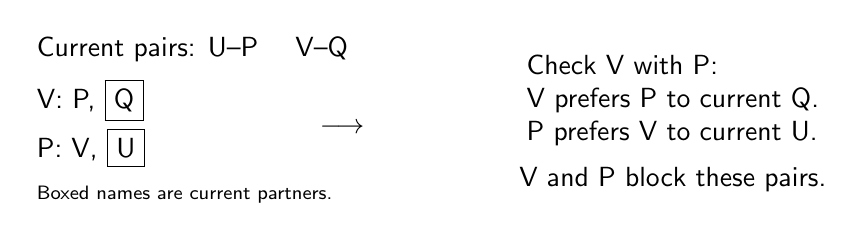
\begin{tikzpicture}[x=1cm,y=1cm]
\node[anchor=west] at (0,1.2){Current pairs: U--P \quad V--Q};
\node[anchor=west] at (0,0.55){V: P, \fbox{Q}};\node[anchor=west] at (0,-0.05){P: V, \fbox{U}};
\node[anchor=west,font=\scriptsize] at (0,-0.65){Boxed names are current partners.};
\node at (4.0,0.2){$\longrightarrow$};
\node[align=left] at (8.2,0.55){Check V with P:\\V prefers P to current Q.\\P prefers V to current U.};
\node at (8.2,-0.45){V and P block these pairs.};
\end{tikzpicture}
\end{center}
\problem{1}{Pair A, B, C with X, Y, Z using these lists. Each pair's score is the sum of its two rank numbers: first choice is 1, second 2, third 3. Add the three pair scores. Which pairing has the lowest total? Is it stable? Find the lowest total among stable pairings.}
\begin{center}\strips{Y, Z, X}{Y, X, Z}{X, Y, Z}{B, A, C}{A, C, B}{B, A, C}\end{center}
\begin{tabular}{|p{2.15in}|p{0.8in}|p{2.15in}|}\hline Pairs&Total&Blocking pair, if any\\\hline\rule{0pt}{32pt}&&\\\hline\rule{0pt}{32pt}&&\\\hline\rule{0pt}{32pt}&&\\\hline\rule{0pt}{32pt}&&\\\hline\rule{0pt}{32pt}&&\\\hline\rule{0pt}{32pt}&&\\\hline\end{tabular}
\lines{2}
\newpage
A missing name is an unacceptable partner. A pair is allowed only when both lists name each other. Every allowed partner is preferred to being unpaired. Leave unpaired objects visible while checking whether both would prefer an allowed new pair.
\problem{2}{Find the stable pairings for each set of lists. Can changing the stable pairing change which objects stay unpaired? A dash means no acceptable choice.}
\begin{center}
\begin{tabular}{r|l@{\hspace{1.2in}}r|l}A&X&X&A, B\\[8pt]B&X&Y&--\end{tabular}
\end{center}
\begin{tabular}{|p{2.65in}|p{2.65in}|}\hline Pairs&Unpaired objects\\\hline\rule{0pt}{44pt}&\\\hline\rule{0pt}{44pt}&\\\hline\end{tabular}
\vspace{20pt}
\begin{center}\strips{X, Y}{Y, X}{Y}{B, A}{A, B, C}{--}\end{center}
\begin{tabular}{|p{2.65in}|p{2.65in}|}\hline Pairs&Unpaired objects\\\hline\rule{0pt}{44pt}&\\\hline\rule{0pt}{44pt}&\\\hline\rule{0pt}{44pt}&\\\hline\end{tabular}
\lines{4}
\newpage
\problem{3}{Pair four objects within one group, using each object once. For each set of lists, find a stable pairing or explain why every pairing has a blocking pair.}
\begin{center}
\begin{tabular}{r|l@{\hspace{1.2in}}r|l}A&B, C, D&A&B, C, D\\[8pt]B&C, A, D&B&A, C, D\\[8pt]C&A, B, D&C&D, A, B\\[8pt]D&A, B, C&D&C, A, B\end{tabular}
\end{center}
\vspace{12pt}
\roommateboard\hfill\roommateboard\hfill\roommateboard
\par\vspace{15pt}
\roommateboard\hfill\roommateboard\hfill\roommateboard
\vspace{16pt}
\lines{6}
\newpage
\problem{4}{Make lists for A, B, C and X, Y, Z, with some names omitted. Can you find two stable pairings that leave different objects unpaired? Find them, or explain why this cannot happen. Keep every allowed partner above being unpaired.}
\begin{center}
\begin{tabular}{r|p{1.8in}@{\hspace{0.6in}}r|p{1.8in}}A&\rule{0pt}{30pt}&X&\\\hline B&\rule{0pt}{30pt}&Y&\\\hline C&\rule{0pt}{30pt}&Z&\\\hline\end{tabular}
\end{center}
\vspace{10pt}
\begin{tabular}{|p{2.65in}|p{2.65in}|}\hline Pairs&Unpaired objects\\\hline\rule{0pt}{52pt}&\\\hline\rule{0pt}{52pt}&\\\hline\end{tabular}
\vspace{16pt}
\lines{8}
\end{document}
